\item \textbf{{[}YIJC/PRELIM/9569/2020/P1/Q6{]} }

A Web Developer is designing an online Sales portal for a company.
The customer needs to submit an online form to register before ordering
through the portal. 
\begin{center}
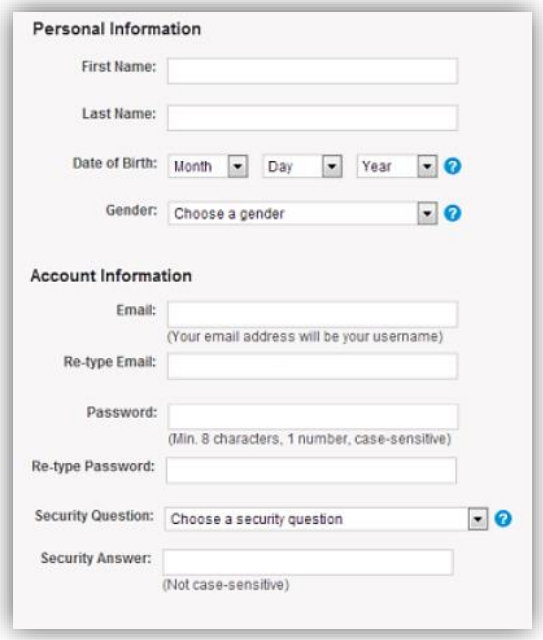
\includegraphics[width=0.25\paperwidth]{C:/Users/Admin/Desktop/Github/question_bank/LyX/static/img/9569-YIJC-2020-P1-Q6}
\par\end{center}
\begin{enumerate}
\item Explain the difference between data validation and data verification.
\hfill{}{[}2{]}
\item Describe two validation checks that the above form should perform
for the customer's inputs.\hfill{} {[}2{]}
\item Describe, with a specific example, how the customer's inputs are being
verified. \hfill{}{[}2{]}
\end{enumerate}
The web developer intends to use CAPTCHA for the above form 
\begin{center}
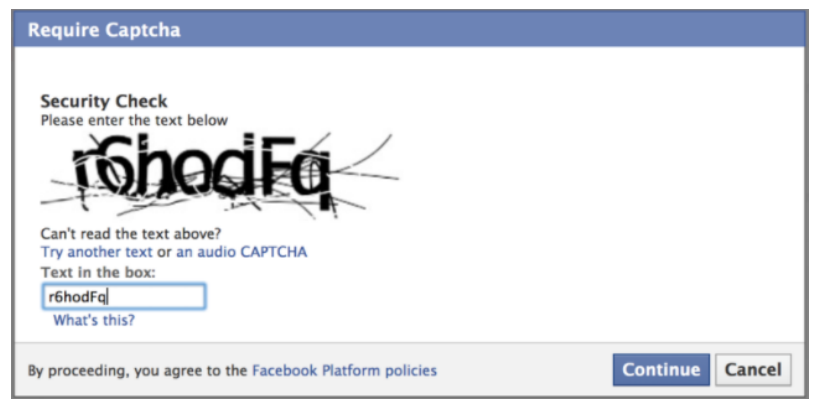
\includegraphics[width=0.3\paperwidth]{C:/Users/Admin/Desktop/Github/question_bank/LyX/static/img/9569-YIJC-2020-P1-Q6-2}
\par\end{center}
\begin{enumerate}
\item Explain what this added feature helps to verify. \hfill{}{[}2{]}
\item Describe the required server scripting to process the customer's input
on his email address and password. \hfill{}{[}4{]}
\item Describe the differences between a web application and a native application.
Explain how the developer should decide between designing a web or
a native application.\hfill{} {[}4{]}
\end{enumerate}